\chapter{Tilanhallinnan ongelmat} \label{Tilanhallinnan ongelmat}

Sovelluksen kasvaessa suuremmaksi ja monimutkaisemmaksi alkaa tilanhallinnassa esiintymään lähestulkoon väistämättä erilaisia esteitä ja vaikeuksia \cite{kentcdodds1} \cite{ivakop}. Tilanhallinnan ongelmat vaikuttavat hyvin konkreettisesti sovelluksen skaalautuvuuteen ja muutosten tekemiseen tulevaisuudessa. Mikäli tilanhallintaa ei huomioida alusta alkaen, siitä johtuvat ongelmat korostuvat \cite{discussion}.

Tässä luvussa käsitellään kahta tyypillistä tilanhallinnan ongelmaa esimerkkien johdattelemana. Tutkielmaan on tarkoituksella valittu käsiteltäväksi nämä kaksi ongelmatyyppiä, sillä muut tilanhallinnassa esiintyvät ongelmat useimmiten juurtavat juurensa näistä kahdesta ongelmatyypistä.

%%
%% Tilan sijainti komponenttipuussa
%%

\section{Tilan sijainti komponenttipuussa}
\label{Tilan sijainti komponenttipuussa}

Tila on aina sidottu sitä hallinnoivaan komponenttiin. Tästä johtuen kyseisen tilallisen komponentin sijainti komponenttipuussa on erityisen tärkeä, mikäli kyseistä tilaa tarvitaan myös sovelluksen muissa komponenteissa.

%%
%% Kaukana oleva käyttökohde
%%

\subsection{Kaukana oleva käyttökohde}
\label{Kaukana oleva käyttökohde}
Luvussa \ref{Tilan jakaminen muille komponenteille} käsitelty tilan jakaminen lapsikomponentille voi alkaa käymään hyvin työlääksi ja sekavaksi, jos tilaa hyödyntävä lapsikomponentti sijaitsee komponenttipuussa huomattavan monen komponenttikerroksen verran alempana. Prop drilling on epävirallinen nimitys prosessista, jossa kehittäjä jakaa komponentin tilaa usean komponenttikerroksen läpi saavuttaakseen lopulta tilaa hyödyntävän komponentin. Tällaisessa tilanteessa kyseessä olevan kahden komponentin väliin jäävät komponentit eivät itse tarvitse kyseistä tilaa. Tällöin ne ainoastaan kuvan \ref{fig:drilling} mukaisesti vastaanottavat sen propseina jakaakseen sen eteenpäin seuraavalle komponentille. \cite{kentcdodds2}
\begin{figure}[h]
\centering 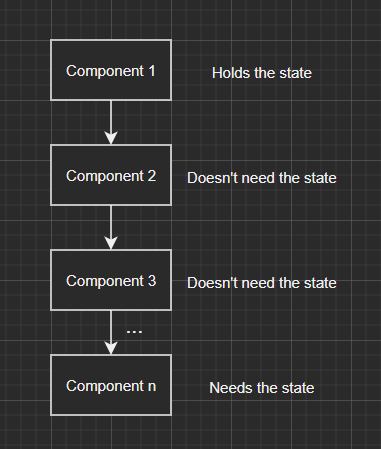
\includegraphics[width=0.5\textwidth]{kuvat/Prop Drilling.png}
\caption{Tilaa voidaan joutua jakamaan usean komponenttikerroksen läpi vaikka väliin jäävät komponentit eivät sitä tarvitse.}
\label{fig:drilling} 
\end{figure}

Sen lisäksi, että prop drilling voi tehdä tilan jakamisesta työlästä, voi myös esimerkiksi mahdollisten muutoksien tekeminen tulevaisuudessa hankaloitua. Mikäli tilaa hallitseva komponentti siirretään tai poistuu kokonaan käytöstä, voi kehittäjä joutua ääritapauksessa purkamaan koko tilaa jakavien komponenttien putken.

%%
%% Jakaminen samalla tasolla
%%

\subsection{Jakaminen samalla tasolla}
\label{Jakaminen samalla tasolla}

Luvussa \ref{Tilan jakaminen muille komponenteille} todettiin, että tieto liikkuu React-sovelluksen komponenttien välillä yksisuuntaisesti ylhäältä alaspäin. Kuitenkin esimerkiksi komponentteja pilkkoessa pienempiin osiin voi kehittäjällä tulla vastaan tilanne, jossa samassa tasossa sijaitsevat komponentit tarvitsevat viereisessä komponentissa hallinnoitua tilaa.
\inputminted[bgcolor=black]{jsx.py:JsxLexer -x}{listaukset/horizontalstate.js}
Esimerkissä esitetty laskuri sisältää kaksi komponenttia, joista \texttt{Counter} sisältää laskurin toiminnallisuuden. \texttt{Display} vastaa laskurin tilan arvon näyttämisestä käyttäjälle. Komponentit ovat komponenttipuussa samalla tasolla, joten tilaa ei voi suoraan jakaa \texttt{Counter}-komponentista \texttt{Display}-komponentin näytettäväksi.

%%
%% Monimutkainen tila
%%

\section{Monimutkainen tila}
\label{Monimutkainen tila}

Yksinkertaisen laskurin ylläpitämän tilan \texttt{count} lukuarvon ylläpitäminen ei ole hankalaa. Laskurin tilan arvoa on helppo muuttaa lisäämällä tai vähentämällä edellisestä arvosta luvun yksi. Laskuria on myös suhteellisen helppoa jatkokehittää esimerkiksi lisäämään tai vähentämään arvoja käyttäjän syötteen perusteella. Jos kyseessä on kuitenkin laskuria huomattavasti monimutkaisempi tietotyyppi tai -rakenne, voi tilan päivittäminen hankaloitua ja täten muuttua jatkokehityksen näkökulmasta huomattavasti työläämmäksi.
\inputminted[bgcolor=black,samepage]{jsx.py:JsxLexer -x}{listaukset/complexstate.js}
Esimerkissä tila \texttt{state} on JavaScript-olio, joka sisältää merkkijonon, kokonaisluvun sekä mielivaltaisen määrän olioita sisältävän taulukon. Esimerkissä käytettyä ES6-standardin mukana tullutta \texttt{spread}-operaattoria käyttämällä päivittäminen on vielä suhteellisen helppoa. Jos kuitenkin halutaan päivittää tilassa esiintyvää arvoa monimutkaisemmalla logiikalla tai useasti toistuvalla tavalla, alkaa tilan päivittämisestä tulla kasvavassa määrin työläämpää. Kehittäjä voi tällaisessa tilanteessa joutua toistuvasti kirjoittamaan logiikaltaan hyvin samankaltaista koodia, jossa ei ole hyödynnetty abstraktiota juuri ollenkaan. Tällainen kehittäminen ei noudata ohjelmistokehityksessä hyväksi todettua DRY-periaatetta (sanoista don't repeat yourself) \cite{dry1} \cite{dry2}.